

\tikzset{every picture/.style={line width=0.75pt}} %set default line width to 0.75pt        

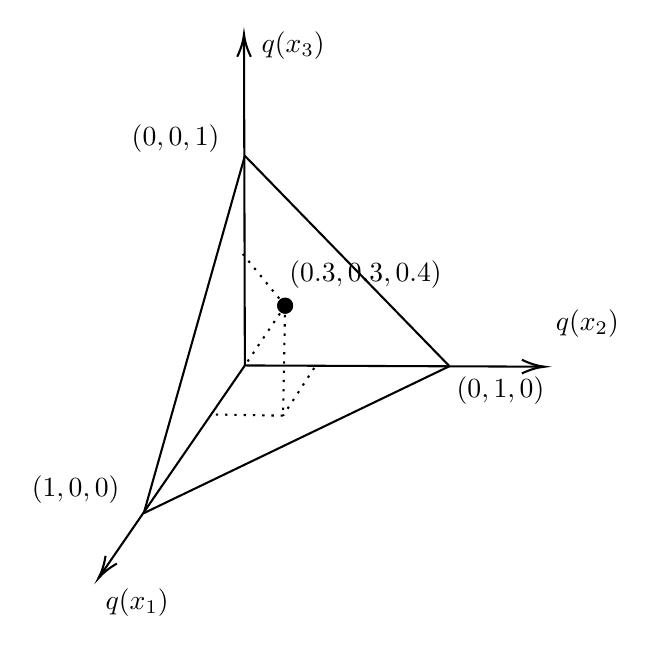
\begin{tikzpicture}[x=0.75pt,y=0.75pt,yscale=-1,xscale=1]
%uncomment if require: \path (0,300); %set diagram left start at 0, and has height of 300

%Straight Lines [id:da4811961842799346] 
\draw    (291,160) -- (433.4,160.59) ;
\draw [shift={(435.4,160.6)}, rotate = 180.24] [color={rgb, 255:red, 0; green, 0; blue, 0 }  ][line width=0.75]    (10.93,-3.29) .. controls (6.95,-1.4) and (3.31,-0.3) .. (0,0) .. controls (3.31,0.3) and (6.95,1.4) .. (10.93,3.29)   ;
%Straight Lines [id:da6300223042341528] 
\draw    (291,160) -- (290.58,2.36) ;
\draw [shift={(290.57,0.36)}, rotate = 89.85] [color={rgb, 255:red, 0; green, 0; blue, 0 }  ][line width=0.75]    (10.93,-3.29) .. controls (6.95,-1.4) and (3.31,-0.3) .. (0,0) .. controls (3.31,0.3) and (6.95,1.4) .. (10.93,3.29)   ;
%Straight Lines [id:da01784826832279296] 
\draw    (291,59) -- (242.29,231.18) ;
%Straight Lines [id:da7686510742972223] 
\draw  [dash pattern={on 0.84pt off 2.51pt}]  (310.4,131.2) -- (291,160) ;
\draw [shift={(310.4,131.2)}, rotate = 123.96] [color={rgb, 255:red, 0; green, 0; blue, 0 }  ][fill={rgb, 255:red, 0; green, 0; blue, 0 }  ][line width=0.75]      (0, 0) circle [x radius= 3.35, y radius= 3.35]   ;
%Straight Lines [id:da16127370523309326] 
\draw    (389.57,160.36) -- (242.29,231.18) ;
%Straight Lines [id:da7110341851384705] 
\draw  [dash pattern={on 0.84pt off 2.51pt}]  (310.4,131.2) -- (309.4,184.2) ;
%Straight Lines [id:da8370462180463676] 
\draw  [dash pattern={on 0.84pt off 2.51pt}]  (324.4,161.2) -- (309.4,184.2) ;
%Straight Lines [id:da4732858000215452] 
\draw  [dash pattern={on 0.84pt off 2.51pt}]  (309.4,184.2) -- (274.4,183.6) ;
%Straight Lines [id:da94953068701914] 
\draw  [dash pattern={on 0.84pt off 2.51pt}]  (310.4,131.2) -- (290,106.3) ;
\draw [shift={(310.4,131.2)}, rotate = 230.67] [color={rgb, 255:red, 0; green, 0; blue, 0 }  ][fill={rgb, 255:red, 0; green, 0; blue, 0 }  ][line width=0.75]      (0, 0) circle [x radius= 3.35, y radius= 3.35]   ;
%Straight Lines [id:da2602355880270242] 
\draw    (291,59) -- (389.57,160.36) ;
%Straight Lines [id:da4136838309775477] 
\draw    (291,160) -- (221.53,260.95) ;
\draw [shift={(220.4,262.6)}, rotate = 304.53] [color={rgb, 255:red, 0; green, 0; blue, 0 }  ][line width=0.75]    (10.93,-3.29) .. controls (6.95,-1.4) and (3.31,-0.3) .. (0,0) .. controls (3.31,0.3) and (6.95,1.4) .. (10.93,3.29)   ;

% Text Node
\draw (235,42.4) node [anchor=north west][inner sep=0.75pt]    {$( 0,0,1)$};
% Text Node
\draw (391.57,163.76) node [anchor=north west][inner sep=0.75pt]    {$( 0,1,0)$};
% Text Node
\draw (186.86,211.82) node [anchor=north west][inner sep=0.75pt]    {$( 1,0,0)$};
% Text Node
\draw (311,108.24) node [anchor=north west][inner sep=0.75pt]    {$( 0.3,0.3,0.4)$};
% Text Node
\draw (297.57,-2.24) node [anchor=north west][inner sep=0.75pt]    {$q( x_{3})$};
% Text Node
\draw (222.4,266) node [anchor=north west][inner sep=0.75pt]    {$q( x_{1})$};
% Text Node
\draw (439.29,131.58) node [anchor=north west][inner sep=0.75pt]    {$q( x_{2})$};


\end{tikzpicture}


    \caption{Example of probability simplex for \(\Omega = \{1, 2, 3\}\) and \(q(1) = 0.2\), \(q(2) = 0.5\), \(q(3) = 0.3\).}
 
%%% Local Variables:
%%% mode: latex
%%% TeX-master: "../main"
%%% End:
